\chapter{Background}
\renewcommand{\baselinestretch}{\mystretch}
\label{chap:BG}
%\setlength{\parindent}{0pt}

\section{Vixen overview}

\PARstart{T}{he} Vixen application \ca{is} based on \ca{the} Microsoft Windows .NET runtime library \cite{platt2002introducing}, developed with \ca{the} C\# programming language \cite{hejlsberg2003c} using Microsoft Visual Studio \cite{msvs}. It is capable of loading modules as dynamic-link libraries (DLL) during runtime. Most of its components such as controllers, lighting effects and editor were implemented as separate modules. \fref{fig:vixen-main} shows the main application interface.

\begin{figure}[!t]
  \centering
  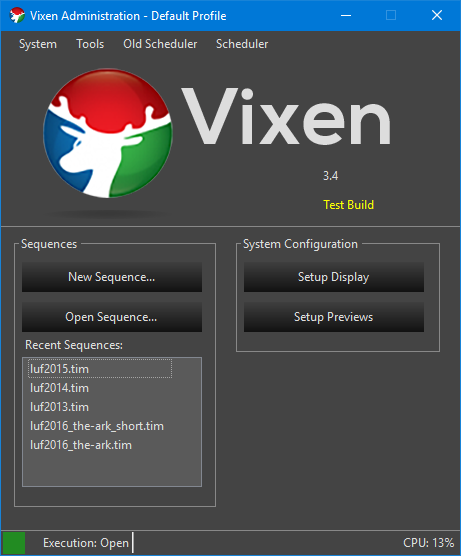
\includegraphics[width=0.6\textwidth]{Figs//vixen_main.png}
  \caption{\footnotesize Main entry GUI of Vixen application}
  \label{fig:vixen-main}
\end{figure}

The execution engine consists of \ca{four} stages for flexible and intuitive lighting sequence editing, as shown in \fref{fig:stages}.

\begin{figure}[!t]
  \centering
  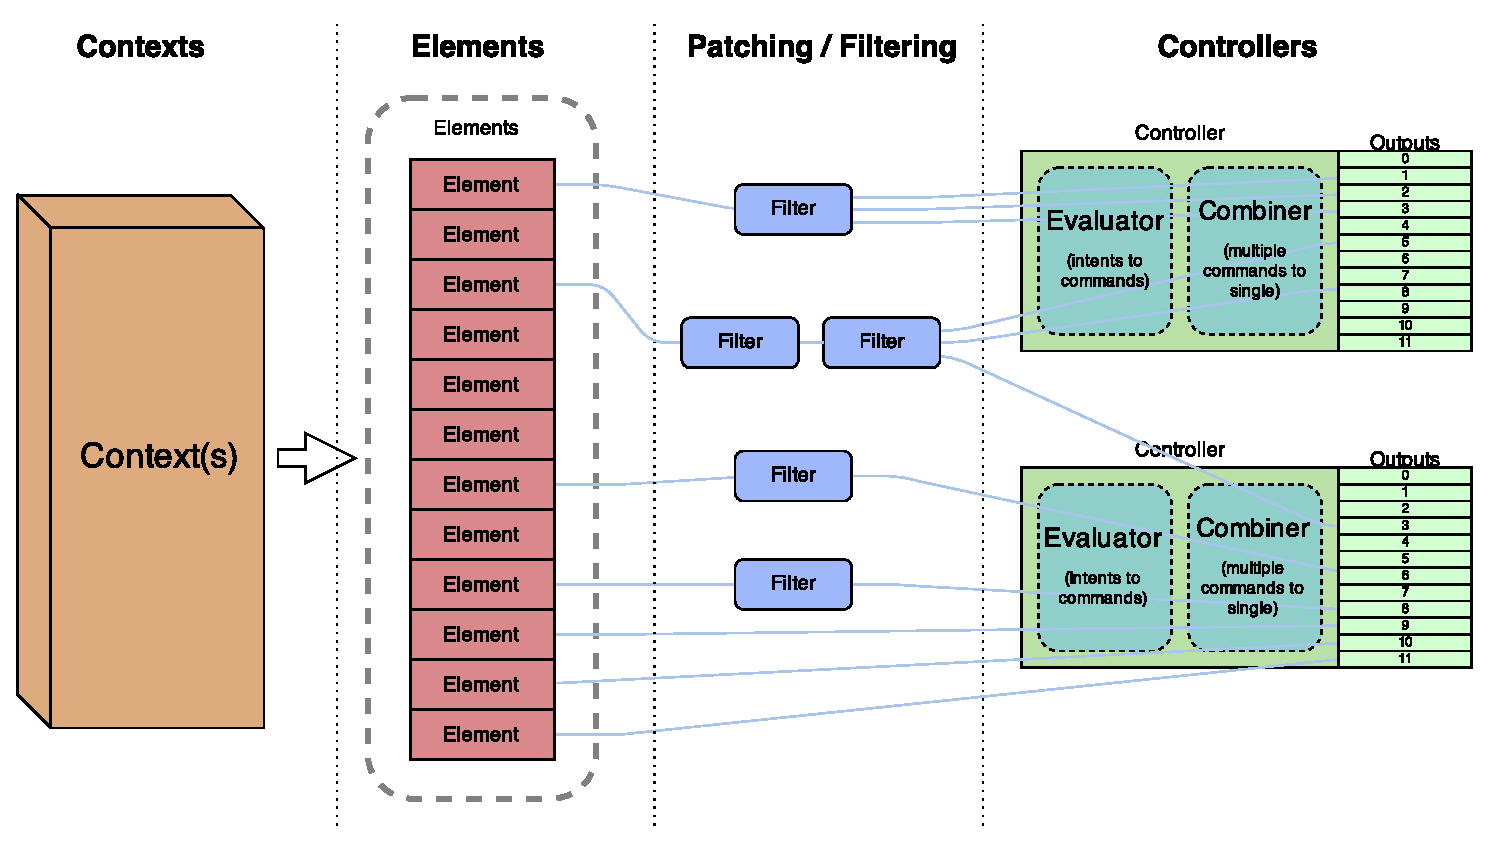
\includegraphics[width=0.85\textwidth]{Figs//V3-Engine-1.eps}
  \caption{\footnotesize Vixen execution engine stages (reproduced from \cite{vixen})}
  \label{fig:stages}
\end{figure}

Contexts are at the very top level of data structures used by Vixen. Vixen stores lighting effects \ca{as} sequence files\ca{;} each sequence represents a context to be executed. By using a built-in show scheduler, Vixen can load, pre-render and cache multiple sequence contexts at the same time, then \ca{schedule them} to be repeatedly played afterwards.

Each sequence context contains lots of elements. Elements represent abstract items described by the user. For example, lights on trees, lights on roofs, etc. They describe the visual display setup, independent of hardware controller connections. Elements can also be grouped together for management and some more advanced display effects. Vixen has a vary flexible sequence designing interface with timeline and audio support, as shown \ca{in} \fref{fig:vixen-editor}.

\begin{figure}[!t]
  \centering
  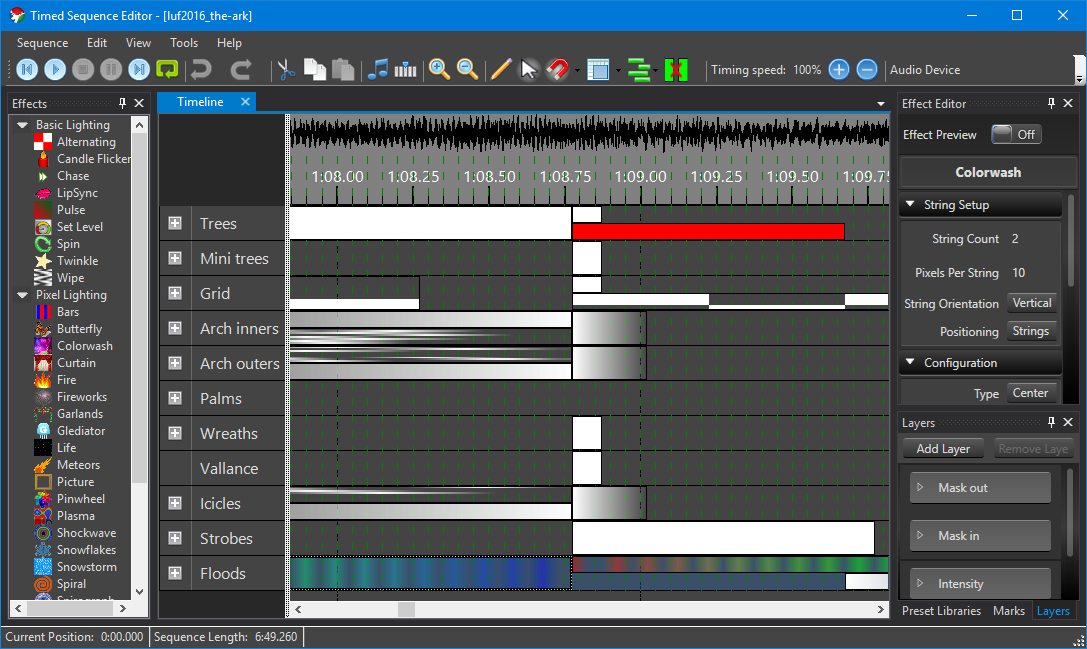
\includegraphics[width=0.9\textwidth]{Figs//vixen_editor.png}
  \caption{\footnotesize Vixen sequence editor interface}
  \label{fig:vixen-editor}
\end{figure}

Between elements and hardware controllers, \ca{patching configurations} are used to map \cad{the} channel connections, \ca{with optional filters inserted between connections}. Each element output may be discarded, duplicated or combined by the filters.

Inside each hardware controller module, data from multiple channels will be combined into a single data packet, then \ca{sent} through the appropriate hardware interface, which can be USB, Ethernet, etc. Each controller has its own update thread, with individual update frame rate settings.

Vixen has another dedicated configuration interface for controllers and filter connections, as shown \ca{in} \fref{fig:vixen-setup}.

\begin{figure}[!t]
  \centering
  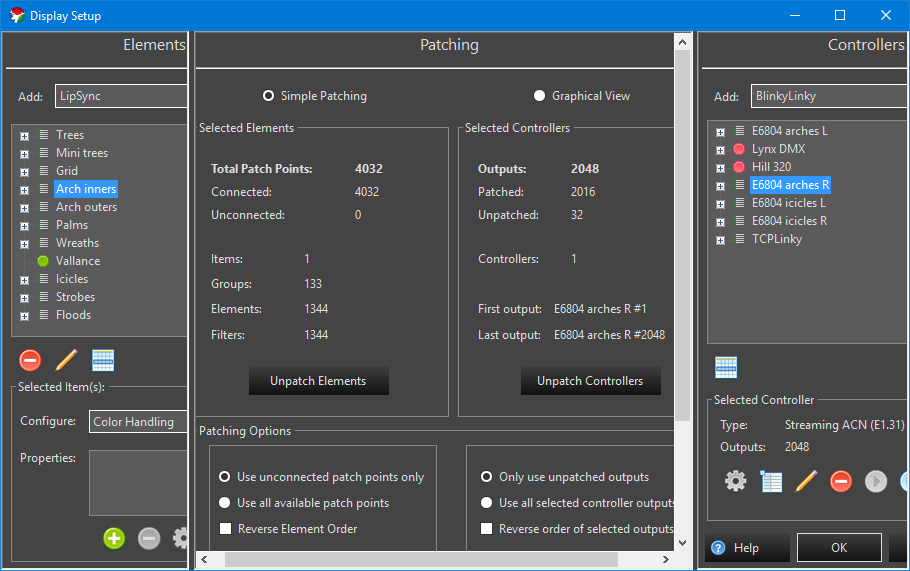
\includegraphics[width=0.9\textwidth]{Figs//vixen_setup.png}
  \caption{\footnotesize Vixen controller setup interface}
  \label{fig:vixen-setup}
\end{figure}

Vixen also has a preview display. It maps element outputs to sets of points on a 2D surface, possibly arranged as the shapes of actual physical objects. The preview \ca{is} rendered \ca{in} a separate window, as shown \ca{in} \fref{fig:vixen-preview}.

\begin{figure}[!t]
  \centering
  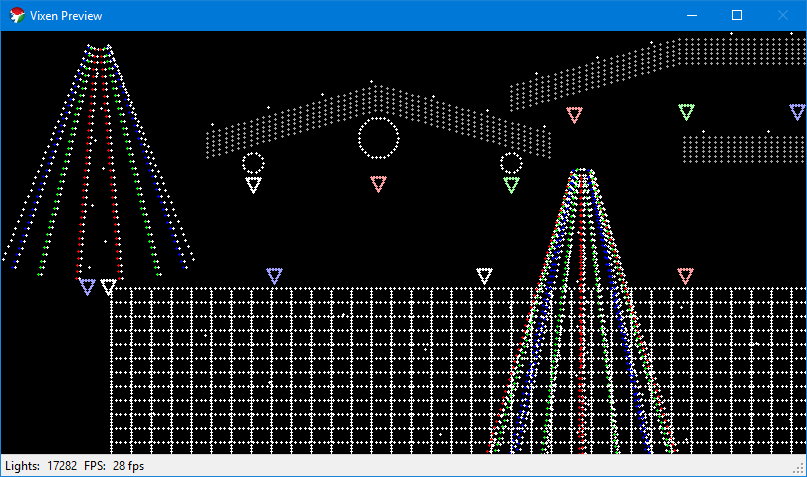
\includegraphics[width=0.9\textwidth]{Figs//vixen_preview.png}
  \caption{\footnotesize Vixen preview interface}
  \label{fig:vixen-preview}
\end{figure}

The Vixen application also features a show scheduler to automatically start \cb{predefined lighting sequences} at \cb{specific times}. Before the shows can be started, the scheduler \cb{needs} to pre-process all scheduled items first. Sequences \ca{using} the original execution engine need \cb{pre-rendering processes}, which can take a significant amount of time.

\section{Similar applications}

\ca{
  There are a few other lighting show companies at the present: Light-O-Rama \cite{lightorama}, SyncroLight \cite{syncrolight} and Revival Control Systems \cite{revival}. Their proprietary software suites \cb{have multiple variants of licenses available} from free basic version up to \$189.95 unlimited version with different channel number limitations, and are all Microsoft Windows only, requiring a computer to work with. Their supported controller types are limited, and also have limitations on lighting effects supported by different controllers. By being proprietary, the exact details of their show engines are not possible to obtain.

The Light-O-Rama software suite has a sequence downloader utility that can only be used with its own customised controllers. After downloaded the sequence, the controller can run in stand-alone mode independently from the computer. From the sequence size optimisation notes, it is most likely using channel intensity levels dumped per frame when intensity changes are present.

Similarly, SyncroLight has a show player with limited controller support for Raspberry Pi. To use it, the show \cb{needs} to be exported to their own \texttt{SHP} file format as the input. It is most likely also a channel data dump.

Vixen also has a sequence export function for a few controller types, as shown in \fref{fig:vixen_export}. However, the objective of this project is to develop an optimised playback engine, not restricted to certain controller types.
}

\section{Testing platforms}

\subsection{Microsoft \ca{Windows-based} systems}

As the Vixen application was originally developed based on Microsoft Windows, \cad{so} a mid-range laptop running Microsoft Windows 10 x64 was used as the primary development platform. It is capable of running Microsoft Visual Studio \ca{as} required for developing the Vixen application, but \ca{has} relatively \ca{low computational} power\ca{, exposing} the run-time performance issue of Vixen.

This platform was also used to remotely connect to other development platforms, using technologies such as SSH.

The hardware specifications are listed below:

\begin{enumerate}[noitemsep,label={}]
  \item CPU: Intel dual-core i5-3337U, 1.80 GHz
  \item RAM: LPDDR3 8.0GB 1600MHz
\end{enumerate}

\subsection{\ca{Linux-based} systems}
\label{sec:systems}

Multiple \ca{Linux-based} systems with a variety of resource configurations, ranging from high performance desktop platforms to low-end embedded platforms, were used for performance testing, as listed in \tref{tbl:linux}. \ca{The laptop running Microsoft Windows also has a Linux system installed, and is listed in the table.}

\begin{table}[t]
  \centering
  \begin{tabular}{l|l|l|l|l}
    \hline
    \textbf{Name} & \textbf{Platform} & \textbf{CPU} & \textbf{Specification} & \textbf{RAM} \\ \hline
    \hline
    NAS         & x86\_64 & AMD FX-8350       & 8 cores @ 4.0 GHz   & 16 GiB  \\ \hline
    Laptop      & x86\_64 & Intel i5-3337U    & 2 cores @ 1.80 GHz  & 8 GiB   \\ \hline
    Jetson TX2  & aarch64 & NVIDIA Tegra X2   & 6 cores @ 2.0 GHz   & 8 GiB   \\ \hline
    RPi 3B      & armv7l  & Broadcom BCM2837  & 4 cores @ 1.2 GHz   & 1 GiB   \\ \hline
    RPi Zero W  & armv6l  & Broadcom BCM2835  & 1 core @ 1.0 GHz    & 512 MiB \\ \hline
    RPi B       & armv6l  & Broadcom BCM2835  & 1 core @ 900 MHz    & 512 MiB \\ \hline
    Noah NP1380 & mipsel  & Ingenic JZ4740    & 1 core @ 336 MHz    & 64 MiB  \\ \hline
  \end{tabular}
  \caption{\footnotesize \ca{Linux-based} systems}
  \label{tbl:linux}
\end{table}

It is possible to install Microsoft Windows IoT \cad{system} on some of the testing platforms. However, system, driver and runtime support were still not available for all of the testing platforms. Therefore, \ca{Debian-based} \cite{debian} Linux distributions of Debian stretch \cite{debian}, Ubuntu xenial \cite{ubuntu} or Raspbian jessie \cite{raspbian} were used on these systems.

\section{Microsoft .NET runtime}

\subsection{Microsoft \ca{Windows-based}}

Most modules included with Vixen were also based on Microsoft's .NET runtime and C\#, with the exception of a few dependency libraries written in C \cite{kernighan1988c} or C++ \cite{stroustrup1995c++} for optional functionality such as audio playback.

Part of the Vixen GUI relies on \ca{the} DirectX interface \cite{directx} and some legacy fragments of Windows Presentation Foundation (WPF) \cite{wpf}. Fortunately, the core functionality of Vixen does not require these components, \ca{making} it possible to be ported to \ca{Linux-based} systems.

\subsection{\ca{Linux-based}}

There were \ca{three} possible ways to run Vixen on \ca{Linux-based} systems:

\begin{enumerate}[noitemsep]
  \item Virtual machine emulation such as qemu \cite{qemu}
  \item Windows runtime emulation such as wine \cite{wine}
  \item Alternative .NET runtime implementation such as mono project \cite{de2004mono}
\end{enumerate}

Virtual machine emulation using qemu was possible on all testing platforms. However, emulation of x86 architecture on non-native ARM platforms requires instruction level emulation, which will be not be feasible \ca{given} the computational power of the available systems. In addition, the entire Microsoft Windows operating system \ca{would} also need to be emulated, further increasing the overhead even on native x86 platforms.

The overhead of running another operating system can be eliminated by using runtime emulators such as wine. However, runtime emulators require x86 platforms for running the x86 based Vixen application, \ca{which is} not possible on \ca{ARM-based} embedded platforms.

The only \ca{feasible} solution was to \ca{use} the mono project runtime implementation. \ca{The} mono project is an up-to-date open source implementation of Microsoft .NET framework using C\#. It can translate executables developed using .NET framework directly to the host platform architecture during runtime, with techniques including Just-in-time (JIT) \ca{compilation}. The functionalities of the executable will be JIT compiled as native code for the host. With the help of other native libraries, the overhead of using mono \ca{runtime} will be insignificant. \ca{Furthermore}, mono project is available to a variety of processor architectures, including ARM and MIPS embedded platforms. Having Vixen running on an embedded platform can give greater flexibility \ca{than a heavy desktop computer or laptop}.

\section{Codec libraries}

Since the overall process of \ca{a} Vixen lighting show is similar to video rendering, to support video format input, a multimedia codec library \ca{needed} to be used for decoding media files. It is impractical to implement numerous video decoding algorithms for different video formats in the time frame of this project, using an existing library would \ca{greatly extend format compatibility with extensively optimised and tested implementations}.

For cross-platform support, an open source implementation would be more suitable. The most popular libraries are \texttt{ffmpeg} \cite{ffmpeg} and \texttt{mencoder} in \texttt{mplayer} \cite{mplayer}. The \texttt{ffmpeg} framework was chosen over \texttt{mplayer}, because it was more actively maintained with \ca{various} hardware acceleration capabilities.

\ca{The \texttt{ffmpeg} framework is originally licensed under the GNU LGPL \cite{lgpl}. However, because several other optional parts that are covered by the GNU GPL \cite{gpl} were incorporated into the \texttt{ffmpeg} framework and were used in this project, especially the \texttt{libx264} library \cite{libx264} for \texttt{h264} encoding, the GPL applies to all of \texttt{ffmpeg}. Fortunately, because the Vixen application itself is open sourced and the library binaries \ca{were} used directly without modification to the source code, this should not \ca{violate} GPL compliance.}

The \texttt{ffmpeg} framework consists of several individual libraries that \ca{were used together in} this project, as listed in \tref{tbl:ffmpeg}.

\begin{table}[t]
  \centering
  \begin{tabular}{l|l}
    \hline
    \textbf{Name} & \textbf{Description} \\ \hline
    \hline
    libavcodec & Encoding/decoding library  \\ \hline
    libavfilter & Graph-based frame editing library \\ \hline
    libavformat & I/O and muxing/demuxing library   \\ \hline
    libavdevice & Special devices muxing/demuxing library \\ \hline
    libavutil & Common utility library    \\ \hline
    libswresample & Audio resampling, format conversion and mixing  \\ \hline
    libpostproc & Post processing library \\ \hline
    libswscale & Colour conversion and scaling library  \\ \hline
  \end{tabular}
  \caption{\footnotesize Different libraries provided by ffmpeg framework (sourced from \cite{ffmpeg})}
  \label{tbl:ffmpeg}
\end{table}

\section{Popular video encoding formats}

There are multiple format \ca{type specifications} for a single video file. First of all, a video container format will be needed to encapsulate \ca{multiple} streams of \ca{different} data \ca{types in a generic video file}. \ca{Such streams may be video streams, audio streams and/or subtitle text streams}. These formats specify how data elements are stored inside a single file, but \ca{do} not specify the encoding or compression format used by individual data streams. Some examples of this type of \ca{format} includes \texttt{mp4} \cite{mp4}, \texttt{avi} \cite{avi} and \texttt{mkv} \cite{mkv}.

For \ca{a} video data stream, another set of encoding formats is used, \cb{such as} \texttt{h264} \cite{h264} and \texttt{mpeg} \cite{mpeg}. In addition, colour space and colour channels will \ca{also need to} be specified. This is known as pixel format. It is often specified by combining colour channels, channel sizes and channel ordering together. The \ca{two} most common colour spaces are \texttt{YUV} (luminance and chrominance) and \texttt{RGB} (red, green and blue). For example, pixel format \texttt{yuv444p} specifies colour space \texttt{YUV} with \texttt{Y} and \texttt{UV} channels taking 12 bytes per 4 pixels, and the channels are stored separately as planes. Similarly, pixel format \texttt{yuv420p} specifies \texttt{YUV} colour space with channels taking 6 bytes per 4 pixels, whereas \texttt{rgb24} specifies \texttt{RGB} colour space with \texttt{R}, \texttt{G} and \texttt{B} channels stored sequentially taking 3 bytes pre pixel.

\section{Audio rendering engine}

Unlike Microsoft Windows\ca{, which has a} definitive audio API, Linux has multiple audio libraries such as \texttt{PulseAudio} \cite{developers2013pulseaudio} and \texttt{ALSA} \cite{alsa} with complex audio framework \ca{structures}. To simplify the underlying structure and enable cross-platform capability, the \texttt{FMOD} \cite{fmod} low-level API library was used. Despite being proprietary, it is available across Windows, Linux and also \ca{ARM-based} embedded platforms with unified easy-to-use API.

The original Vixen application already uses \texttt{FMOD} as a plugin in the original execution engine. However, the version it uses was \ca{outdated} without \ca{documentation available}, and the plugin is only capable of playing audio files. Therefore, a more recent version was required. Furthermore, although the library has provided a set of C\# APIs, \cad{but} the essential functionality required for playing custom audio stream was lacking, C/C++ APIs \ca{needed} to be used \ca{instead}.

\section{Performance analysers}

Several performance analysers on different platforms \ca{were} used \ca{throughout} the project for optimisation and debugging \ca{purposes}.

On Microsoft Windows, the built-in sampling profiler for Visual Studio was used. It samples the stack frame multiple times during runtime without significant impact to program performance, analyses execution frequencies and \ca{durations} of individual functions.

On Linux, the mono project also has \ca{a profiler} with sampling mode for \ca{analysing} code segments that were written with C\# using .NET runtime. Linux also has sampling profilers for native programs, especially the \texttt{perf} profiler \cite{de2010new}. However, they \ca{cannot} provide much information about code written with intermediate languages such as C\# with .NET runtime. \ca{The mono profiler \cb{was} used for most of the C\# implementations in this project, while \texttt{perf} was used occasionally for native libraries.}

\section{Performance profiling method}

In addition to profilers provided by the platform, performance profiling was also implemented within the Vixen application itself. It has relatively less overheads from generic profiling tools. However, it can only provide information specifically related to the execution engine, such as controller update frame rates. Therefore, the profiler was used only for overall execution performance comparison of the Vixen application.

The original profiler with Vixen uses the \texttt{Process} class provided by Microsoft Windows runtime for CPU usage measurements. However, it was not completely available under mono runtime. A different profiling method would be required for Linux.

On Linux, there are statistic files in the \texttt{proc} file system \cite{proc} provided by the kernel. Per-process information about CPU jiffies \ca{(time unit defined by the interval of system timer) and} disk I/O statistics are available by reading corresponding files.
